\ifx\wholebook\relax\else
\documentclass{report}
\usepackage{times}
\usepackage{epsfig}
\usepackage{alltt}
\usepackage{xspace}
\usepackage{graphicx}
\usepackage{ifpdf}
\usepackage{ifthen}
\usepackage{amsmath}
\usepackage{a4wide}

\graphicspath{{figures/}} 

\ifpdf
\DeclareGraphicsExtensions{.pdf, .jpg, .tif, .png}
\else
\DeclareGraphicsExtensions{.eps, .jpg}
\fi

\newboolean{toseecomment}
\setboolean{toseecomment}{false}
%%change to false to hidde comment 
\newcommand{\comment}[1]{\ifthenelse{\boolean{toseecomment}}{$\blacktriangleright$ \textit{#1}$\blacktriangleleft$}{}}

\newcommand{\commented}[1]{}

\newboolean{seevwspecific}
\setboolean{seevwspecific}{true}
\newcommand{\vwspecific}[1]{\ifthenelse{\boolean{seevwspecific}}{#1}{}}

\newboolean{seecategoryspecific}
\setboolean{seecategoryspecific}{false}
\newcommand{\categoryspecific}[1]{\ifthenelse{\boolean{seecategoryspecific}}{#1}{}}

\newboolean{seestorespecific}
\setboolean{seestorespecific}{true}
\newcommand{\storespecific}[1]{\ifthenelse{\boolean{seestorespecific}}{#1}{}}

\newboolean{seesqueakspecific}
\setboolean{seesqueakspecific}{false}
\newcommand{\squeakspecific}[1]{\ifthenelse{\boolean{seesqueakspecific}}{#1}{}}


\newcommand{\category}[0]
{\ifthenelse{\boolean{seestorespecific}}
	{package\xspace}
	{category\xspace}}

\newcommand{\ct}[1]{\texttt{#1}\xspace}
\newcommand{\stc}[1]{{\small {\sf #1}}\xspace}
\newcommand{\ST}{{\textsc Smalltalk}\xspace}
\newcommand{\tab}{\makebox[4em]{}}
\newcommand{\ttt}[1]{{\tt #1}}
\newcommand{\chev}{\ttt{>>}}
\newcommand{\vw}{VisualWorks\xspace}
\newcommand{\sq}{Squeak\xspace}
\newcommand{\store}{Store\xspace}
\renewcommand{\chaptername}{Exercise}
\newcommand{\exercise}{\vspace{0.2cm}\noindent \textbf{Exercise:}\xspace}

\newsavebox{\fminibox}
\newlength{\fminilength}

% Fait un truc encadre
\newenvironment{fminipage}[1][\linewidth]
  {\setlength{\fminilength}{#1-2\fboxsep-2\fboxrule}
        \begin{lrbox}{\fminibox}\begin{minipage}{\fminilength}}
  { \end{minipage}\end{lrbox}\noindent\fbox{\usebox{\fminibox}}}

% Pareil mais pas encadre (a utiliser pour ne pas couper une fonction

\newenvironment{nminipage}[1][\linewidth]
  {\setlength{\fminilength}{#1}
        \begin{lrbox}{\fminibox}\begin{minipage}{\fminilength}}
  { \end{minipage}\end{lrbox}\noindent\mbox{\usebox{\fminibox}}}

% Un alltt encadre
\newenvironment{falltt}
  {\vspace*{0.3cm}\begin{fminipage}\begin{alltt}}
  {\end{alltt}\end{fminipage}\vspace*{0.3cm}}

% Un alltt pas encadre
\newenvironment{nalltt}
  {\vspace*{0.3cm}\begin{nminipage}\begin{alltt}}
  {\end{alltt}\end{nminipage}\vspace*{0.3cm}}

% Une fonction encadree
\newenvironment{ffonction}[1]
  {\begin{fonction}[#1]
        \begin{fminipage}
\begin{alltt}
\rule{\linewidth}{0.5pt}}
{\end{alltt}\end{fminipage}\end{fonction}}

\newenvironment{codeonepage}
  {\begin{nminipage}\vspace*{0.2cm}\hrule\vspace*{0.1cm}
\begin{alltt}}
  {\end{alltt} \vspace*{-0.2cm}\hrule \vspace*{0.2cm} \end{nminipage}}

\newenvironment{code}
  {\vspace*{0.1cm}\hrule\vspace*{-0.1cm}\begin{alltt}}
  {\end{alltt}\vspace*{-0.2cm}\hrule \vspace*{0.1cm}}


\begin{document}
\fi

% $Author: ducasse $
% $Date: 2005/05/16 13:38:16 $
% $Revision: 1.1.1.1 $


\newcommand{\job}[1]{\vspace{7 pt}\noindent \textbf{Your job:}~#1 \vspace{7 pt}}
\newcommand{\regconf}{RegConf}

\chapter{A Simple Application for Registering to a Conference}
\mainauthor{\bergel}

\metadata{Squeak}{Squeak/VisualWorks}{?www.squeaksource.com/RegConf?}{?1.2?}{bergel@iam.unibe.ch}

%%%%%% %%%%%% %%%%%% %%%%%% %%%%%% %%%%%% %%%%%% %%%%%%
The goal of this tutorial is to give you a feeling on creating a web application using Seaside. \regconf~is  a tool intended to help people to register to a conference. 

\section{RegConf: An Application for Registering to a Conference}

\sd{What is the application doing?}

Four steps are necessary to complete a registration:
\begin{enumerate}
\item A participant has to enter some personal data such as firstname, name, the institute where she is attached, and her email address.
\item Then some information about the hotel are required. For instance a room can be single or double in an hotel ranked between 1 and 4 stars. A price has then to be computed.
\item Finally informations regarding the payment are required. Once the credit card number, the issue date, and the type are entered,
\item A confirmation screen shows a summary of what was entered.
\end{enumerate}



The flow of the application is described in the following figure.

\begin{figure}
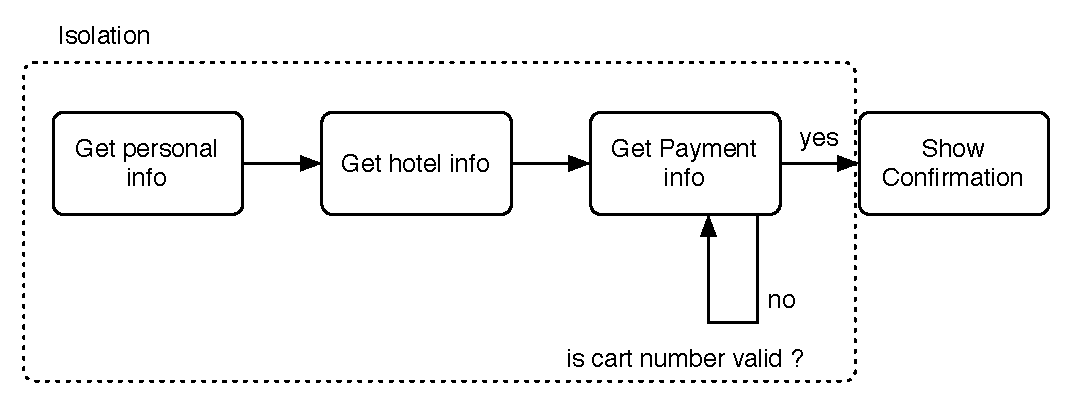
\includegraphics[scale=0.7]{flow}
\caption{}
\end{figure}

The dashed rectangle designate the part of the application which is \textit{isolated}. This means that once the flow of the running application leaves this box, there is no way to come back in it, specially using the back button.

%%%%%% %%%%%% %%%%%% %%%%%% %%%%%% %%%%%% %%%%%% %%%%%%

\section{Application Building Blocks}

\subsection{The Entry Point: \ct{RCMain}}
The control flow of the application has to be described in a task's \ct{go} method. This method also represent the entry point of the application. Thus a name like \ct{RCMain} sounds appropriated (\ct{RC} stands for \regconf). 

\job{Create a task \ct{RCMain} with a \ct{go} method that describes the control flow of the application.}

\job{Start the web server on by executing \ct{WAKom startOn: 9090}.}

\job{Create an \ct{initialize} method on the class side to register your application in Seaside under the name \ct{regconf}.}


\subsection{Getting User Information: \ct{RCGetUserInfo}}

All the control flow is defined in the class you previously defined. Getting user information is implemented as a normal seaside component (i.e., subclass of \ct{WAComponent}). Instance variables of this class should reflect the structure of a user. Pressing the \textit{submit} button returns to the caller component using \ct{answer:}. Fetching the participant's informations can be done using text fields and submit button. Here is an example:

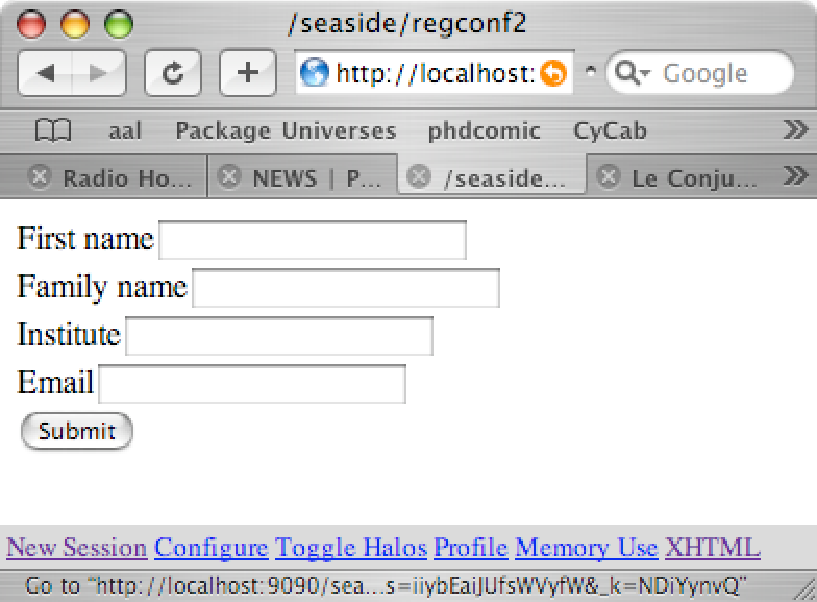
\includegraphics[scale=0.7]{userinfo}

\job{Write the method \ct{renderContentOn:} in \ct{RCGetUserInfo}.}

\job{Try your application using your favorite web browser. Make it point to \ct{http://localhost:9090/seaside/regconf}.}

The information passed around different states of the application can be contained in a dictionary. A more advanced design would require a class \ct{User} for which an instance is passed around through.

\subsection{Getting Hotel Information: \ct{RCGetHotelInfo}}
A list of choices is pleasant to fetch informations of the hotel. 

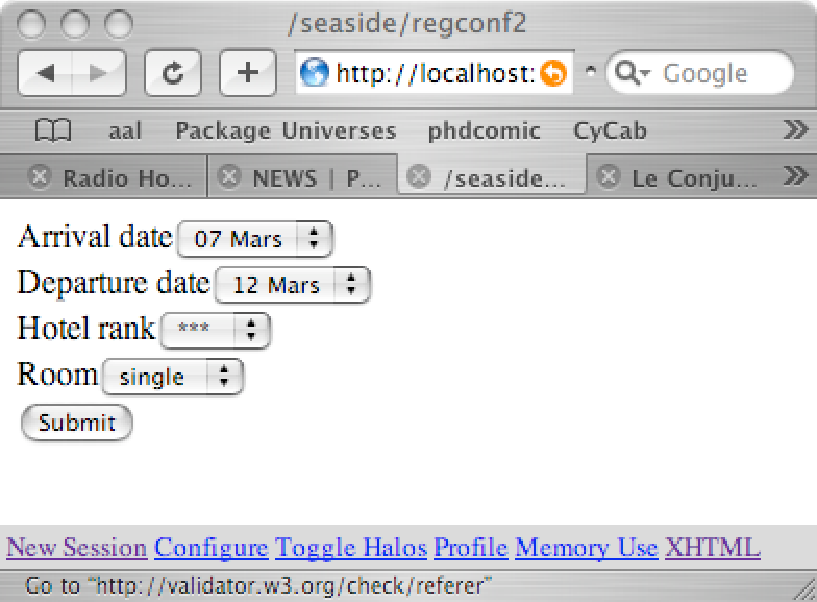
\includegraphics[scale=0.7]{hotel}

\job{Write the class \ct{RCGetHotelInfo}}



\subsection{Payment: \ct{RCPayment}}
The payment is valid only if 16 number was provided and if the issue date is not over.

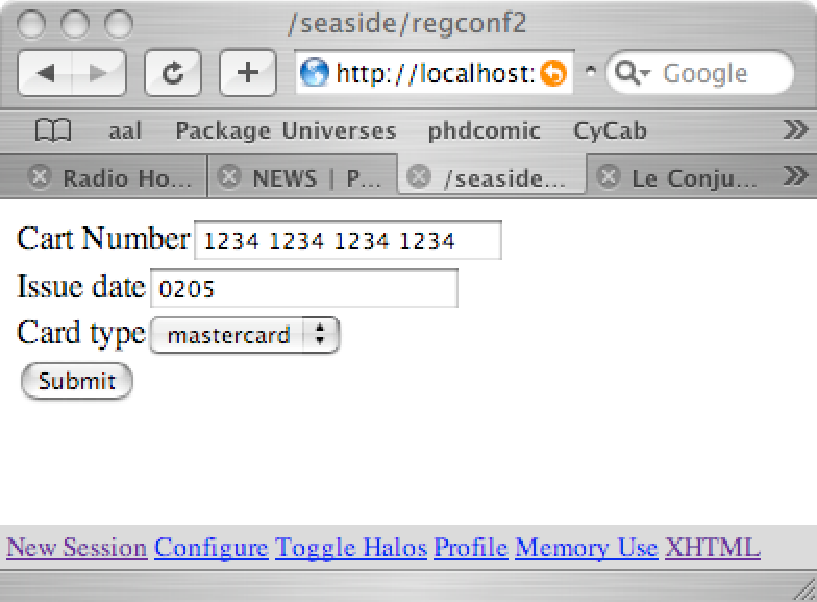
\includegraphics[scale=0.7]{creditcard}

\job{Write the class \ct{RCPayment}}

\subsection{Confimation: \ct{RCConfirmation}}
Once the payment is done, it is nice to show a summary of what was done.

\job{Write the class \ct{RCConfirmation}}


\section{Extensions}
\job{Study the class MiniCalendar of Seaside. Create a calendar starting from today.}
\job{Use the mini calendar to add the possibility to say when and until which day the person wants to keep the room.}



\ifx\wholebook\relax\else\end{document}\fi